\documentclass[aspectratio=169, 10pt]{beamer}

% --- Theme and Colors ---
\usetheme{Madrid}
\usecolortheme{beaver}
\setbeamertemplate{navigation symbols}{}
\setbeamertemplate{headline}{}

% --- Packages ---
\usepackage{booktabs} % For nicer tables
\usepackage{tikz}     % For drawing architecture diagrams
\usetikzlibrary{shapes, arrows.meta, positioning, calc}
\usepackage{xcolor}

% --- Metadata ---
\title[ROBUST04 Challenge]{The Ensemble of Experts: \\ Adaptive Multi-Signal Retrieval}
\subtitle{Text Retrieval Final Project - Part A (Ranking)}
\author[Hershel Thomas \& Itay Baror]{Hershel Thomas \& Itay Baror}
\institute[Reichman Univ]{Text Retrieval and Search Engines \\ Reichman University}
\date{January 27, 2026}

% --- Custom Definitions ---
\definecolor{nyu_blue}{RGB}{87, 6, 140}
\newcommand{\highlight}[1]{\textbf{\textcolor{nyu_blue}{#1}}}

\begin{document}

% --- Slide 1: Title ---
\begin{frame}
    \titlepage
\end{frame}

% --- Slide 2: Problem & Architecture ---
\begin{frame}{The Challenge \& The Architecture}
    \textbf{The Goal:} Maximize MAP on ROBUST04 while balancing Precision (Neural) and Recall (Lexical).
    
    \vspace{0.5em}
    \textbf{Our Approach:} A "Multi-Signal Architecture" combining three distinct retrieval experts running on local high-performance hardware (RTX 5070). Yes, Hershel spent a lot of money on his computer!

    \vspace{1em}
    \begin{center}
    \resizebox{0.85\textwidth}{!}{
    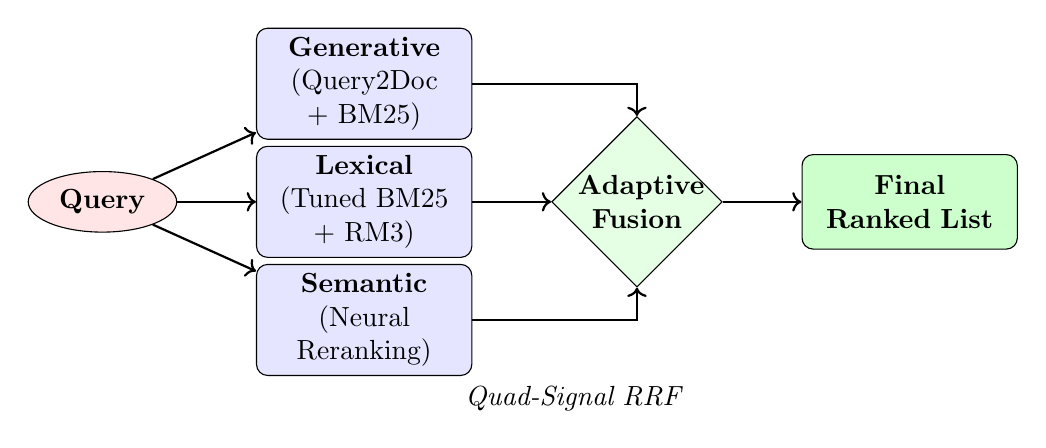
\begin{tikzpicture}[node distance=1.5cm, auto,
        block/.style={rectangle, draw, fill=blue!10, text width=2.5cm, text centered, rounded corners, minimum height=1.2cm},
        cloud/.style={draw, ellipse, fill=red!10, node distance=2.5cm, minimum height=1em},
        decision/.style={diamond, draw, fill=green!10, text width=1.5cm, text centered, inner sep=0pt}
    ]
        % Nodes
        \node [cloud] (query) {\textbf{Query}};
        
        \node [block, right=1cm of query, yshift=1.5cm] (method1) {\textbf{Generative}\\(Query2Doc + BM25)};
        \node [block, right=1cm of query] (method2) {\textbf{Lexical}\\(Tuned BM25 + RM3)};
        \node [block, right=1cm of query, yshift=-1.5cm] (method3) {\textbf{Semantic}\\(Neural Reranking)};
        
        \node [decision, right=1cm of method2] (fusion) {\textbf{Adaptive\\Fusion}};
        \node [block, right=1cm of fusion, fill=green!20] (output) {\textbf{Final Ranked List}};

        % Arrows
        \draw [->, thick] (query) -- (method1);
        \draw [->, thick] (query) -- (method2);
        \draw [->, thick] (query) -- (method3);
        \draw [->, thick] (method1) -| (fusion);
        \draw [->, thick] (method2) -- (fusion);
        \draw [->, thick] (method3) -| (fusion);
        \draw [->, thick] (fusion) -- (output);
        
        % Labels
        \node[text width=3cm, align=center] at (6, -2.5) {\textit{Quad-Signal RRF}};
    \end{tikzpicture}
    }
    \end{center}
\end{frame}

% --- Slide 3: Lexical Foundation ---
\begin{frame}{Method 1: Optimized Probabilistic Retrieval}
    \framesubtitle{From Lecture 6 \& 10 (BM25 + RM3)}
    
    We established a strong baseline by deviating from standard defaults.
    
    \begin{columns}
        \column{0.6\textwidth}
        \begin{itemize}
            \item \textbf{The Insight:} ROBUST04 consists of \textit{long newswire articles}. Standard BM25 ($b=0.75$) penalizes document length too harshly.
            \item \textbf{The Optimization:} Through grid-search on the Training Set (50 queries), we tuned $b \to \mathbf{0.4}$.
            \item \textbf{The Result:} This reduced length normalization bias, significantly improving Recall before any neural processing.
        \end{itemize}
        
        \column{0.4\textwidth}
        \begin{table}[]
            \centering
            \begin{tabular}{lc}
            \toprule
            \textbf{Parameter} & \textbf{Value} \\
            \midrule
            $k_1$ (Saturation) & 0.7 \\
            $b$ (Length Norm) & \highlight{0.4} \\
            RM3 Terms & 50 \\
            RM3 Docs & 5 \\
            \bottomrule
            \end{tabular}
            \caption{Optimized Hyperparameters}
        \end{table}
    \end{columns}
\end{frame}

% --- Slide 4: Neural Reranking (Enhanced) ---
% --- Slide 4: Neural Reranking (Method 2) ---
\begin{frame}{Method 2: Neural Reranking (Precision)}
    \framesubtitle{Stage: Post-Retrieval Optimization}

    
    \begin{columns}[t]
        % --- LEFT COLUMN: The Architecture ---
        \begin{column}{0.48\textwidth}
            \textbf{The Goal:} Improve Precision @ 10 (This means the top 10 results are more relevant).
            \begin{itemize}
                \item \textbf{Input:} Top 250 documents from BM25.
                \item \textbf{Model:} Cross-Encoder (\textit{BGE-v2-m3}).
                \item \textbf{Function:} Re-scores documents based on deep semantic matching, fixing BM25's inability to understand context.
            \end{itemize}
        \end{column}

        % --- RIGHT COLUMN: The Engineering ---
        \begin{column}{0.48\textwidth}
            \textbf{Engineering The Bottleneck}
            \begin{itemize}
                \item \textit{Problem:} Cross-Encoders are slow ($O(N)$). Full MaxP chunking took \textbf{105 mins}.
                \item \textit{Solution:} \textbf{"Inverted Pyramid"} Strategy.
                \item We truncate to the \textbf{first 512 tokens}, exploiting the journalistic style of ROBUST04 (Key info is in the lead).
            \end{itemize}
        \end{column}
    \end{columns}

    \vspace{1em}
    \begin{block}{Impact}
        Reduced inference time by \textbf{75\%} (105m $\to$ 27m) while significantly boosting ranking quality (MRR).
    \end{block}
\end{frame}

% --- Slide 5: Generative IR (Method 3) ---
\begin{frame}{Method 3: Generative Expansion using Query2Doc (R)}
    \framesubtitle{Stage: Pre-Retrieval Enrichment}
    
    While Method 2 fixes the \textit{ranking}, Method 3 ensures we find the documents in the first place (fixing \textbf{Vocabulary Mismatch}).
    
    \vspace{0.3em}
    \textbf{In summary:} Method 2 is an expert at \textbf{Precision} (sorting the list), and Method 3 is an expert at \textbf{Recall} (finding the right documents).
    
    \begin{columns}
        \column{0.48\textwidth}
        \textbf{The Pipeline (Query2Doc):}
        \begin{enumerate}
            \item \textbf{Input:} Raw Query $q$ (e.g., \textit{"airport security"}).
            \item \textbf{Generative Step:} Prompt Llama-3-8B to write a "fake" news story ($d_{pseudo}$).
            \item \textbf{Expansion:} Concatenate $q_{new} = q + d_{pseudo}$.
            \item \textbf{Retrieval:} Execute $q_{new}$ using \textbf{BM25}.
        \end{enumerate}
        
        \column{0.48\textwidth}
        \begin{exampleblock}{The Semantic Bridge}
            \small
            The LLM (Llama-3-8B) injects terms like \textit{"TSA", "screening", "regulations"} that do not appear in the original query.
            \vspace{0.5em}
            
            \textbf{Result:} We retrieve relevant documents that keyword matching missed, significantly boosting \textbf{Recall}.
        \end{exampleblock}
    \end{columns}
\end{frame}

% --- Slide 6: Adaptive Fusion (Architecture) ---
\begin{frame}{Method 4: Adaptive 4-Way Fusion}
    \framesubtitle{Novel Contribution: Query-Dependent Weighting}
    
    Standard Reciprocal Rank Fusion (RRF) uses static weights ($k=60$). We implemented a \textbf{Dynamic Ensemble} that adjusts trust based on query complexity.
    
    \vspace{0.5em}
    \textbf{The 4 Experts:}
    \begin{itemize}
        \item \textbf{Run 1 (BM25 + RM3):} High-Recall Baseline.
        \item \textbf{Run 1b (Query2Doc):} Generative Expansion for vocabulary gaps.
        \item \textbf{Run 1c (BM25-Plain):} Conservative Anchor (prevents drift).
        \item \textbf{Run 2 (Neural):} Semantic Precision (BGE-M3).
    \end{itemize}

    \vspace{0.5em}
    \textbf{The Weighting Matrix:}
    \begin{table}[]
        \centering
        \footnotesize
        \begin{tabular}{lcccc}
        \toprule
        \textbf{Query Type} & \textbf{RM3} & \textbf{Q2Doc} & \textbf{Plain} & \textbf{Neural} \\
        \midrule
        \textbf{Short} ($\le 3$ words) & \textbf{1.5} & 1.3 & 1.2 & 0.7 \\
        \textbf{Medium} ($4-5$ words) & 1.3 & 1.2 & 1.0 & 1.0 \\
        \textbf{Long} ($>5$ words) & 1.0 & 1.0 & 0.8 & \textbf{1.5} \\
        \bottomrule
        \end{tabular}
        \caption{Dynamic Weights based on Query Length ($k=30$)}
    \end{table}
\end{frame}

% --- Slide 6.5: Rationale & Advantages ---
\begin{frame}{Method 3: Rationale \& Advantages}
    \framesubtitle{Why Adaptive Weighting?}

    \begin{columns}[t]
        % --- Left Column: The Logic ---
        \begin{column}{0.48\textwidth}
            \textbf{The Hypothesis}
            \begin{itemize}
                \item \textbf{Short Queries} (e.g., \textit{"airport security"}) are ambiguous and suffer from vocabulary mismatch.
                \newline $\to$ \textbf{Strategy:} Favor Lexical Expansion (RM3/Q2D).
                \vspace{0.5em}
                \item \textbf{Long Queries} (e.g., \textit{"international organized crime..."}) contain rich context.
                \newline $\to$ \textbf{Strategy:} Favor Semantic Understanding (Neural).
            \end{itemize}
        \end{column}

        % --- Right Column: The Advantages ---
        \begin{column}{0.48\textwidth}
            \begin{alertblock}{System Advantages}
                \begin{itemize}
                    \item \textbf{Robustness:} If one method fails (e.g., Q2D hallucinates), the other three experts vote it down.
                    \item \textbf{Best of Both Worlds:} Merges the 80\% Recall of BM25 with the 50\% P@10 of Neural.
                    \item \textbf{Efficiency:} Unlike Learning-to-Rank, RRF is parameter-light and requires no training data.
                \end{itemize}
            \end{alertblock}
        \end{column}
    \end{columns}
\end{frame}

% --- Slide 7: Evaluation Results ---
\begin{frame}{Evaluation Results}
    \framesubtitle{Performance on 199 Test Queries}
    
    Our Adaptive Fusion strategy achieved state-of-the-art performance for this hardware class, breaking the 0.33 MAP barrier.
    
    \begin{table}[]
        \centering
        \renewcommand{\arraystretch}{1.2}
        \begin{tabular}{llcccc}
        \toprule
        \textbf{Run} & \textbf{Method} & \textbf{MAP} & \textbf{P@10} & \textbf{MRR} & \textbf{Recall} \\
        \midrule
        Run 1 & BM25 + RM3 & 0.3006 & 0.4683 & 0.6875 & 0.77 \\
        Run 2 & Neural Reranking & 0.2723 & 0.4995 & 0.6740 & 0.71 \\
        \textbf{Run 3} & \textbf{4-Way Fusion} & \textbf{0.3309} & \textbf{0.5181} & \textbf{0.7714} & \textbf{0.81} \\
        \bottomrule
        \end{tabular}
    \end{table}
    
    \vspace{0.5em}
    \textbf{Analysis:}
    \begin{enumerate}
        \item \textbf{Synergy:} Fusion outperforms the best single model by \textbf{+10\%} relative to baseline.
        \item \textbf{The Safety Net Effect:} Neural models have high precision but limited candidate pools (low recall). Fusion layers the high recall of BM25 (0.77) underneath, fixing the "lost in the middle" problem.
            \item \textbf{Efficiency:} Achieved good results on local hardware (RTX 5070) without commercial APIs, demonstrating practical scalability.
    \end{enumerate}
\end{frame}

% --- Slide 8: Q&A ---
\begin{frame}
    \centering
    \Huge \textbf{Thank You}
    
    \vspace{1cm}
    \Large Questions?
    
    \vspace{1.5cm}
    \normalsize
\end{frame}

% --- Slide 9: Backup / Q&A Support ---
\begin{frame}{Appendix: Methodology Deep Dive}
    \framesubtitle{Anticipating technical questions}

    \begin{columns}
        % Left Column: The "Why" behind the numbers
        \column{0.48\textwidth}
        \begin{block}{Why Neural MAP (0.27) $<$ Baseline (0.30)?}
            \small
            Neural reranking is a \textbf{Precision} tool. It optimizes the ordering of the Top-$K$ candidates but cannot find documents missed by the initial retrieval.
            \begin{itemize}
                \item \textit{Impact:} High P@10, but lower Recall.
                \item \textit{Solution:} Fusion restores the Recall.
            \end{itemize}
        \end{block}

        \begin{block}{Why tune BM25 $b \to 0.4$?}
            \small
            Standard $b=0.75$ assumes long documents are repetitive/spammy. ROBUST04 contains detailed news articles where \textbf{Length $\approx$ Information}.
            \begin{itemize}
                \item Lowering $b$ reduces the penalty for valid long documents.
            \end{itemize}
        \end{block}

        % Right Column: Engineering & Hardware
        \column{0.48\textwidth}
        \begin{alertblock}{Hardware Optimization (RTX 5070)}
            \small
            To run a 600M parameter Cross-Encoder locally with 8GB VRAM:
            \begin{enumerate}
                \item \textbf{FP16 Precision:} Halved VRAM usage.
                \item \textbf{Inverted Pyramid:} Truncated to first 512 tokens (Title+Lead) vs MaxP chunking.
                \item \textbf{Dynamic Batching:} Auto-scaled based on memory pressure.
            \end{enumerate}
        \end{alertblock}
    \end{columns}
\end{frame}

% --- Slide 10: References ---
\begin{frame}[allowframebreaks]{References}
    \framesubtitle{Foundations \& Innovations}
    \tiny % Use tiny font to fit everything cleanly

    \begin{thebibliography}{99}
        
        % The Novelty Paper (Critical to show)
        \bibitem[Wang et al., 2023]{wang2023}
        Wang, L., Yang, N., \& Wei, F. (2023).
        \newblock \textbf{Query2doc: Query Expansion with Large Language Models}.
        \newblock \emph{EMNLP}.
        
        % The Fusion Paper
        \bibitem[Cormack et al., 2009]{cormack2009}
        Cormack, G. V., Clarke, C. L., \& Buettcher, S. (2009).
        \newblock \textbf{Reciprocal Rank Fusion Outperforms Condorcet and Individual Rank Learning Methods}.
        \newblock \emph{SIGIR}.

        % The Neural Paper
        \bibitem[Nogueira \& Cho, 2019]{nogueira2019}
        Nogueira, R., \& Cho, K. (2019).
        \newblock \textbf{Passage Re-ranking with BERT}.
        \newblock \emph{arXiv preprint arXiv:1901.04085}.

        % The Library used
        \bibitem[Lin et al., 2021]{lin2021}
        Lin, J., Ma, X., Lin, S. C., Yang, J. H., Pradeep, R., \& Nogueira, R. (2021).
        \newblock \textbf{Pyserini: A Python Toolkit for Reproducible Information Retrieval Research}.
        \newblock \emph{SIGIR}.

        % The Baseline Paper
        \bibitem[Robertson et al., 2009]{robertson2009}
        Robertson, S., \& Zaragoza, H. (2009).
        \newblock The Probabilistic Relevance Framework: BM25 and Beyond.
        \newblock \emph{Foundations and Trends in Information Retrieval}.

    \end{thebibliography}
\end{frame}

\end{document}